\documentclass[20pt]{ctexart}
\usepackage{amsmath, amssymb}
\usepackage{tikz}
\usepackage{geometry}
\usepackage{booktabs}
\usepackage{enumitem}
\geometry{margin=1in}
\usetikzlibrary{arrows.meta}

 \newgeometry{left=0.5cm,bottom=0.1cm}


\newcommand{\overarrow}[1]{\overrightarrow{#1}}
\newcommand{\colvec}[2]{\begin{pmatrix} #1 \\ #2 \end{pmatrix}}

\title{Vectors, Translations, and Meaning}
\author{Extension Sheet}
\date{}

\begin{document}
\maketitle

\section*{1\quad Vector translation review}

Point $A = (2,3)$ is translated by $ \bf{t}=\colvec{4}{1}$. Find the destination.

\vspace{4em}

Apply the same translation to $B = (-1,5)$.

\vspace{5em}

\section*{2 \quad Word embeddings}

AI models take words and assign them coordinates $(x,y)$, so that the words can be processed by algorithms - this is called a \textbf{word embedding}. Below is an example of this for 8 words:

\begin{center}
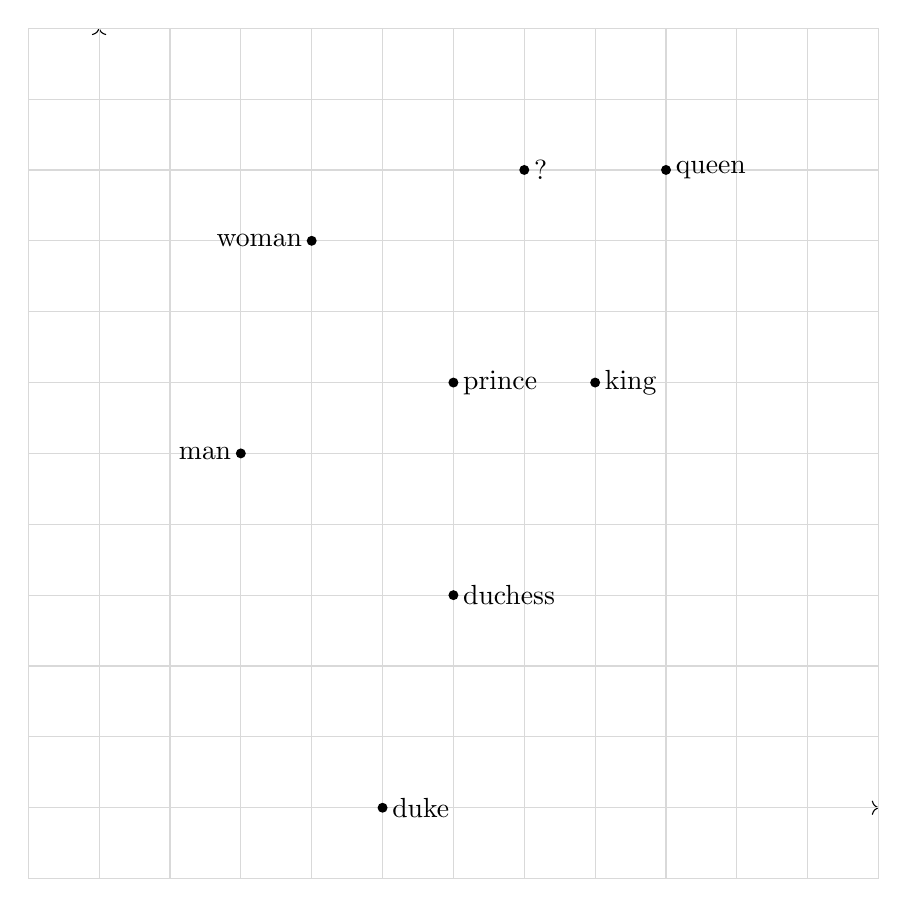
\begin{tikzpicture}[scale=0.9]
  % axes and grid
  \draw[->] (-1,0)--(11,0);
  \draw[->] (0,-1)--(0,11);
  \draw[step=1cm,gray!30] (-1,-1) grid (11,11);

  % semantic cluster (left side)
  \fill (2,5) circle (2pt) node[left] {man};
  \fill (3,8) circle (2pt) node[left] {woman};
  \fill (7,6) circle (2pt) node[right] {king};
  \fill (8,9) circle (2pt) node[right] {queen};
  \fill (5,6) circle (2pt) node[right] {prince};
  \fill (4,0) circle (2pt) node[right] {duke};
  \fill (5,3) circle (2pt) node[right] {duchess};

  % missing princess (dashed)
  \fill (6,9) circle (2pt) node[right] {?};

\end{tikzpicture}
\end{center}

\newpage{}

\begin{enumerate}[label=\textbf{\arabic*.}]
  \item Compute the vector $\overarrow{\text{king}\quad\text{queen}}$. \vspace{5em}
  \item Compute the vector $\overarrow{\text{duke} \quad\text{duchess}}$. \vspace{5em}

  \item What do you think the translation $\colvec{1}{3}$ represents in our word vector embedding?

\vspace{5em}

  \item Consider $\overarrow{\text{man} \quad \text{woman}}$, does that match up with your answer to the previous question?

  \vspace{5em}

  \item What word is missing at the question mark ?
\end{enumerate}

\newpage{}
\section*{3 \quad Translating English to Chinese}

Machine translation is a field of AI that deals with translating text between two different languages, below is an incomplete grid and translation table:




\begin{center}

\begin{tikzpicture}[scale=0.65]
  \draw[step=1cm,gray!50] (-10,-10) grid (15,15);

  \draw[->] (-10,0)--(15,0);
  \draw[->] (0,-10)--(0,15);

  % English cluster
  \fill (9,8) circle (2pt) node[above right] {man};
  \fill (10,11) circle (2pt) node[above right] {?};

  \fill (7,8) circle (2pt) node[above right] {boy};
  \fill (8,11) circle (2pt) node[above right] {girl};
  \fill (8,6) circle (2pt) node[above right] {king};
  \fill (9,9) circle (2pt) node[above right] {?};

  \fill (6,6) circle (2pt) node[above right] {?};
  \fill (7,9) circle (2pt) node[above right] {?};


  % Chinese cluster (shifted)
  \fill (-6,-2) circle (2pt) node[right] {男人};
  \fill (-5,1) circle (2pt) node[right] {?};
  \fill (-6,-1) circle (2pt) node[right]  {王妃};
  \fill (-7,-4) circle (2pt) node[right] {国王};
  

  % gender pair in Chinese
  \fill (-8,-2) circle (2pt) node[right] {?};
  \fill (-7,1) circle (2pt) node[right] {女孩};

  \fill (-9,-4) circle (2pt) node[right] {王子};
  \fill (-9,0) circle (2pt) node[right] {?};



\end{tikzpicture}
\end{center}

\subsection*{Translation table (incomplete)}

\begin{center}
\begin{tabular}{@{}llll@{}}
\toprule
English & English coords & Chinese & Chinese coords \\
\midrule
man     & (9,8)  & 男人 & (-6,-2) \\
woman & (10,11) & 女人 & (-5,1) \\
boy     &  & 男孩 &  \\
 &  & 女孩 & (-7,1) \\
 & (8,6)  & &  \\
 & & 王妃 &  \\
prince & & 王子 &  \\
princess & (7,9) & 公主 & (-9,0)  \\


\bottomrule
\end{tabular}
\end{center}



\subsection*{Tasks}

\begin{enumerate}[label=\textbf{\arabic*.}]

\item Use the given coordinates and table to compute the translation vector $\bf{t}$ from English to Chinese.

\vspace{5em}

\item Fill in the missing values in the table and coordinate grid

\vspace{5em}

\item (Challenge) What do you think the vector $\colvec{-2}{0}$ means in the context of this word-vector embedding?

\vspace{5em}

\item (Challenge) The bottom row of the table does not follow the pattern, why do you think this is? (hint - consider the Chinese characters)

\end{enumerate}

\bigskip

% --------------------
% Teacher answers:
% translation vector T = (4,3) - (9,8) = (-5,-5)
% princess_en = (5,9)
% princess_cn = (5,9) + (-5,-5) = (0,4)
% Chinese word = 公主 (gōngzhǔ)
% --------------------
\newpage
% %======================================================
% \section*{4\quad Parallel vectors}
% %======================================================

% Below is an incomplete grid and translation table

% \vspace{-1em}

% % -------------------------------------------------------
% % Coordinate summary (for reference):
% %
% % Translation vector English -> Chinese:
% %   T = (-14,-12)
% %
% % ENGLISH cluster:
% %   good(2,5)   better(4,7)   best(6,9)
% %   bad(2,2)    4,4   worse(5,4)
% %               6,6    worst(6,5)
% %   tall(9,2)   taller(11,4)
% %   fast(9,6)   faster(11,8)
% %
% % CHINESE cluster  (all shifted left and down by (-4,-4)):
% %   好(-12,-7)   更好(-10,-5)   最好(-8,-3)
% %   坏(-12,-10)  更坏(-10,-8)   最坏(-8,-6)
% %   高(-5,-10)   更高(-3,-8)
% %   快(-5,-6)    更快(-3,-4)
% %
% % Note:
% % English "worse/worst" are irregular.
% % Chinese comparatives are perfectly regular with step (2,2).
% % -------------------------------------------------------

% \begin{center}
% \begin{tikzpicture}[scale=0.6]
%   \draw[step=1cm,gray!30] (-15,-13) grid (13,11);
%   \draw[->] (-15,0)--(13,0) node[right] {$x$};
%   \draw[->] (0,-13)--(0,11) node[above] {$y$};

%   % ------ English cluster ------

%   % good / better / best
%   \fill (2,5)  circle (3pt) node[above left]  {\small good};

%   % ghost regular predictions
%   \draw[dashed,gray!60] (4,7) circle (3pt);
%   \node[gray!70, above right] at (1,7) {\small\itshape ``gooder''?};

%   \draw[dashed,gray!60] (6,9) circle (3pt);
%   \node[gray!70, right] at (6,9) {\small\itshape ``goodest''?};
  
%   \fill (3,6)  circle (3pt) node[above left]  {\small better};
%   \fill (5,7)  circle (3pt) node[above left]  {\small best};

%   % tall / taller
%   \fill (9,2)  circle (3pt) node[below right] {\small tall};
%   \fill (11,4) circle (3pt) node[above right] {\small taller};
%   \fill (13,6) circle (3pt) node[above right] {\small tallest};

%   % fast / faster
%   \fill (9,6)  circle (3pt) node[below right] {\small fast};
%   \fill (11,8) circle (3pt) node[above right] {\small faster};
%   \fill (13,10) circle (3pt) node[above right] {\small fastest};

%   % bad
%   \fill (2,2)  circle (3pt) node[below left]  {\small bad};

%   % ghost regular predictions
%   \draw[dashed,gray!60] (4,4) circle (3pt);
%   \node[gray!70, above right] at (4,4) {\small\itshape ``badder''?};

%   \draw[dashed,gray!60] (6,6) circle (3pt);
%   \node[gray!70, right] at (6,6) {\small\itshape ``baddest''?};

%   % actual worse / worst
%   \fill (5,4)  circle (3pt) node[right] {\small worse};
%   \fill (6,5)  circle (3pt) node[right] {\small worst};

%   % ------ Chinese cluster (shifted by (-4,-4)) ------

%   % 好 family
%   \fill (-12,-7) circle (3pt) node[left] {\small 好};
%   \fill (-10,-5) circle (3pt) node[left] {\small 更好};
%   \fill (-8,-3)  circle (3pt) node[left] {\small 最好};

%   % 坏 family
%   \fill (-12,-10) circle (3pt) node[left] {\small 坏};
%   \fill (-10,-8)  circle (3pt) node[left] {\small 更坏};
%   \fill (-8,-6)   circle (3pt) node[left] {\small 最坏};

%   % 高 family
%   \fill (-5,-10) circle (3pt) node[below left] {\small 高};
%   \fill (-3,-8)  circle (3pt) node[below right] {\small 更高};
%   \fill (-1,-6)  circle (3pt) node[below right] {\small 最高};

%   % 快 family
%   \fill (-5,-6) circle (3pt) node[above left] {\small 快};
%   \fill (-3,-4)  circle (3pt) node[above right] {\small 更快};
%   \fill (-1,-2)  circle (3pt) node[above right] {\small 最快};

% \end{tikzpicture}
% \end{center}

% \begin{center}
% \begin{tabular}{@{}llll@{}}
% \toprule
% English & English coords & Chinese & Chinese coords \\
% \midrule
% tall    & $(9,2)$   & 高   & $(-5,-10)$ \\
% taller  & $(11,4)$  & 更高 & $(-3,-8)$ \\
% tallest & $(11,4)$  & 最高 & $(-3,-8)$ \\
% fast    & $(9,6)$   & 快   & $(-5,-6)$ \\
% faster  & $(11,8)$  & 更快 & $(-3,-4)$ \\
% fastest & $(13,10)$ & 最快 & $(-1,-2)$ \\
% good    & $(2,5)$   & 好   & $(-12,-7)$ \\
% better  & $(3,6)$   & 更好 & $(-10,-5)$ \\
% best    & $(5,7)$   & 最好 & $(-8,-3)$ \\
% bad     & $(2,2)$   & 坏   & $(-12,-10)$ \\
% worse   & $(5,4)$   & 更坏 & $(-10,-8)$ \\
% worst   & $(6,5)$   & 最坏 & $(-8,-6)$ \\
% \bottomrule
% \end{tabular}
% \end{center}

% \newpage{}

% \begin{enumerate}[label=\textbf{\arabic*.}]

% \item Compute $\overarrow{\text{good}\;\text{better}}$ and
% $\overarrow{\text{tall}\;\text{taller}}$ using the coordinates in the grid.
% Are these two vectors parallel? Show your working clearly. \vspace{6em}

% \item The hollow circle labelled \emph{``more bad''?} shows where the regular
% pattern would predict the comparative of \emph{bad}.
% \begin{enumerate}[label=(\alph*)]
%   \item What are the coordinates of that ghost point?
%   \item Compute $\overarrow{\text{bad}\;\text{worse}}$ using the actual position of \emph{worse}.
%   \item By how much does $\overarrow{\text{bad}\;\text{worse}}$ differ from the regular
%   vector $\colvec{2}{2}$?
%   \item Why does English have a different word for the comparative of \emph{bad}
%   rather than using \emph{badder}? What is this linguistic phenomenon called?
% \end{enumerate}
% \vspace{8em}

% \item Now look at \emph{worst}.
% \begin{enumerate}[label=(\alph*)]
%   \item Compute $\overarrow{\text{good}\;\text{best}}$. How does it relate to
%   $\overarrow{\text{good}\;\text{better}}$?
%   \item The hollow circle for \emph{``most bad''?} is at $(6,6)$.
%   Compute $\overarrow{\text{bad}\;\text{worst}}$ using the actual position of \emph{worst}.
%   \item Compare $\overarrow{\text{bad}\;\text{worst}}$ with
%   $\overarrow{\text{good}\;\text{best}}$.
%   By how much do they differ, and in which component?
% \end{enumerate}
% \vspace{8em}

% \item Now look at the Chinese cluster in the bottom-left.
% \begin{enumerate}[label=(\alph*)]
%   \item Compute $\overarrow{\text{坏}\;\text{更坏}}$ and
%   $\overarrow{\text{坏}\;\text{最坏}}$.
%   \item Are these parallel to $\overarrow{\text{好}\;\text{更好}}$?
%   \item Chinese forms comparatives by adding the prefix 更 (gèng, ``more'') and
%   superlatives with 最 (zuì, ``most'') to any adjective without exception.
%   How does this grammatical regularity show up in the geometry of the embedding?
%   Why does the Chinese cluster \emph{not} need any ghost points?
% \end{enumerate}
% \vspace{8em}

% \item Compare $\overarrow{\text{good}\;\text{best}}=\colvec{4}{4}$ with
% $\overarrow{\text{bad}\;\text{worst}}=\colvec{4}{3}$.
% In Chinese, both $\overarrow{\text{好}\;\text{最好}}$ and
% $\overarrow{\text{坏}\;\text{最坏}}$ equal $\colvec{4}{4}$.
% \begin{enumerate}[label=(\alph*)]
%   \item What does this single-unit difference in the English vectors suggest about
%   how the model has ``learned'' that \emph{worse/worst} are irregular?
%   \item (Challenge) Do you think the vectors for \emph{go / went} or \emph{good / well}
%   would be parallel to $\overarrow{\text{fast}\;\text{faster}}$?
%   Explain your reasoning.
% \end{enumerate}
% \vspace{6em}

% \end{enumerate}

% \subsection*{Translation table}

% The translation vector from English to Chinese is
% \[
% \mathbf{T}=\colvec{-14}{-12}.
% \]



% \medskip
% \noindent\textbf{Notice:}
% The Chinese coordinates for \emph{更坏} and \emph{最坏} are obtained
% by applying the regular $(2,2)$ comparative step from 坏,
% \emph{not} by translating the English \emph{worse}/\emph{worst} positions.
% Why do you think these two routes give different answers?

% \vspace{5em}

% In word embeddings, a \emph{direction} often represents a particular kind of change in meaning.
% If the same change applies in many contexts, the vectors will be \textbf{parallel}.

% The grid below shows adjective comparatives in English (top-right cluster) and Chinese
% (bottom-left cluster). Hollow circles mark where the \emph{regular} pattern predicts a word
% should sit; solid circles are where the embedding actually places it.

% \newpage
% %======================================================
% \section*{5\quad Orthogonal directions: independent meanings}
% %======================================================

% In a vector space, two vectors are \textbf{orthogonal} if their dot product is zero.
% Geometrically, they meet at a right angle, and in word embeddings this can signal that
% the two directions represent \emph{independent} aspects of meaning.

% The grid below shows four words.

% \begin{center}
% \begin{tikzpicture}[scale=0.9]
%   \draw[step=1cm,gray!30] (-1,-1) grid (11,11);
%   \draw[->] (-1,0)--(11,0) node[right] {$x$};
%   \draw[->] (0,-1)--(0,11) node[above] {$y$};

%   % four key words
%   \fill (2,2) circle (2pt) node[below right] {boy};
%   \fill (6,2) circle (2pt) node[below right] {man};
%   \fill (2,8) circle (2pt) node[above right] {girl};
%   \fill (6,8) circle (2pt) node[above right] {woman};

%   % arrows for gender direction
%   \draw[->,thick,blue!70] (2,2)--(2,8) node[midway,left] {$\mathbf{g}$};
%   \draw[->,thick,blue!70] (6,2)--(6,8) node[midway,right] {$\mathbf{g}$};

%   % arrows for age direction
%   \draw[->,thick,red!70] (2,2)--(6,2) node[midway,below] {$\mathbf{a}$};
%   \draw[->,thick,red!70] (2,8)--(6,8) node[midway,above] {$\mathbf{a}$};

% \end{tikzpicture}
% \end{center}

% \begin{enumerate}[label=\textbf{\arabic*.}]

%   \item Write down the vectors $\mathbf{g} = \overarrow{\text{boy}\;\text{girl}}$ and
%   $\mathbf{a} = \overarrow{\text{boy}\;\text{man}}$ using the coordinates in the grid.
%   \vspace{5em}

%   \item Compute $\mathbf{g} \cdot \mathbf{a}$.
%   What does the result tell you about the directions \emph{gender} and \emph{age} in this embedding?
%   \vspace{6em}

%   \item Now add the word \texttt{king} at $(6,10)$ and \texttt{queen} at $(2,10)$ to the grid.
%   Compute $\overarrow{\text{man}\;\text{king}}$ and check whether it is orthogonal to $\mathbf{g}$.
%   \vspace{6em}

%   \item Why would it be \emph{useful} for the gender direction and the age/status direction
%   to be orthogonal in a real word embedding?
%   \vspace{5em}

%   \item Give an example of two linguistic features you would \emph{not} expect to be orthogonal
%   in a word embedding, and explain why.
%   \vspace{5em}

% \end{enumerate}


% \newpage
% %======================================================
% \section*{6\quad Linear combinations of meaning vectors}
% %======================================================

% Complex changes in meaning can be built by combining simpler ones.
% The grid below shows five words with their embedding coordinates.

% \begin{center}
% \begin{tikzpicture}[scale=0.82]
%   \draw[step=1cm,gray!30] (-1,-1) grid (13,13);
%   \draw[->] (-1,0)--(13,0) node[right] {$x$};
%   \draw[->] (0,-1)--(0,13) node[above] {$y$};

%   % words
%   \fill (2,2)  circle (2pt) node[below right] {boy};
%   \fill (6,2)  circle (2pt) node[below right] {man};
%   \fill (2,8)  circle (2pt) node[above right] {girl};
%   \fill (6,8)  circle (2pt) node[above right] {woman};
%   \fill (6,12) circle (2pt) node[above right] {queen};

%   % g and s vectors shown from boy
%   \draw[->,thick,blue!70]  (2,2)--(2,8)  node[midway,left]  {$\mathbf{g}$};
%   \draw[->,thick,red!70]   (2,8)--(6,12) node[midway,above left] {$\mathbf{s}$};

%   % dashed route direct boy->queen
%   \draw[->,dashed,gray!60,thick] (2,2)--(6,12);

% \end{tikzpicture}
% \end{center}

% \begin{enumerate}[label=\textbf{\arabic*.}]

%   \item Let $\mathbf{g} = \overarrow{\text{boy}\;\text{girl}}$ and
%   $\mathbf{s} = \overarrow{\text{girl}\;\text{queen}}$.
%   Write $\overarrow{\text{boy}\;\text{queen}}$ in terms of $\mathbf{g}$ and $\mathbf{s}$.
%   \vspace{5em}

%   \item Using coordinates from the grid, verify your answer by computing
%   $\mathbf{g} + \mathbf{s}$ numerically and checking it equals $\overarrow{\text{boy}\;\text{queen}}$.
%   \vspace{6em}

%   \item Could you also write $\overarrow{\text{boy}\;\text{queen}}$ using $\mathbf{a} = \overarrow{\text{boy}\;\text{man}}$
%   and some other vector? Find a second route on the grid and write out the combination.
%   What does having two routes to the same word tell us about the geometry?
%   \vspace{7em}

%   \item The word \texttt{king} sits at $(6,12)$ in this embedding --- the same point as \texttt{queen}.
%   Is that realistic? What might a better embedding do differently to separate them?
%   \vspace{5em}

% \end{enumerate}


% \newpage
% %======================================================
% \section*{7\quad Projection from higher dimensions to 2D}
% %======================================================

% Real word embeddings live in very high-dimensional spaces (often hundreds of dimensions).
% When we draw them on paper we \emph{project} them down to 2D, which can distort relationships.

% \subsection*{A simple 3D embedding}

% Imagine three independent features: \textbf{gender} ($x$-axis), \textbf{age} ($y$-axis), \textbf{status} ($z$-axis).
% Four words are placed in this 3D space:

% \medskip
% \begin{center}
% \begin{tabular}{@{}lrrr@{}}
% \toprule
% Word & $x$ (gender) & $y$ (age) & $z$ (status) \\
% \midrule
% boy    & 0 & 0 & 0 \\
% girl   & 4 & 0 & 0 \\
% man    & 0 & 4 & 0 \\
% king   & 0 & 4 & 4 \\
% \bottomrule
% \end{tabular}
% \end{center}

% \medskip

% \begin{enumerate}[label=\textbf{\arabic*.}]

%   \item Why is a 3D space natural for representing these four words?
%   Which pairs of words differ in exactly one feature?
%   \vspace{5em}

%   \item Below are two 2D projections of the same four points.
%   \textbf{Projection A} drops the $z$-axis (plots $x$ vs $y$).
%   \textbf{Projection B} drops the $x$-axis (plots $y$ vs $z$).
%   Plot all four words on each grid.

% \begin{center}
% \begin{tikzpicture}[scale=0.72]
%   % Projection A: x vs y (drop z)
%   \begin{scope}
%     \draw[step=1cm,gray!30] (-1,-1) grid (7,7);
%     \draw[->] (-1,0)--(7,0) node[right] {\small $x$ (gender)};
%     \draw[->] (0,-1)--(0,7) node[above] {\small $y$ (age)};
%     \node at (3,-0.8) {\textbf{Projection A} (drop $z$)};
%   \end{scope}

%   % Projection B: y vs z (drop x)  -- offset to the right
%   \begin{scope}[xshift=10cm]
%     \draw[step=1cm,gray!30] (-1,-1) grid (7,7);
%     \draw[->] (-1,0)--(7,0) node[right] {\small $y$ (age)};
%     \draw[->] (0,-1)--(0,7) node[above] {\small $z$ (status)};
%     \node at (3,-0.8) {\textbf{Projection B} (drop $x$)};
%   \end{scope}
% \end{tikzpicture}
% \end{center}

%   \vspace{2em}

%   \item In 3D, $\overarrow{\text{boy}\;\text{girl}}$ (along $x$) and $\overarrow{\text{boy}\;\text{king}}$
%   (along $y$ and $z$) are orthogonal.
%   Check this by computing their dot product in 3D.
%   \vspace{5em}

%   \item Now look at Projection A.
%   Are the two arrows still perpendicular on the 2D plot?
%   Does this mean the meanings are no longer independent?
%   Explain your answer.
%   \vspace{6em}

%   \item In Projection B, \texttt{boy} and \texttt{man} map to the same point.
%   What problem does this cause if someone only looks at Projection B?
%   \vspace{5em}

%   \item How does this help explain why different 2D visualisations of the \emph{same}
%   word embedding can look very different from each other?
%   \vspace{5em}

% \end{enumerate}


% \newpage{}

% % ============================================================
% %  Answer-key / reference grid  (same as original last page)
% % ============================================================

% \begin{center}

% \begin{tikzpicture}[scale=0.65]
%   \draw[step=1cm,gray!30] (-10,-10) grid (15,15);

%   \draw[->] (-10,0)--(15,0);
%   \draw[->] (0,-10)--(0,15);

%   % English cluster
%   \fill (9,8) circle (2pt) node[above right] {man};
%   \fill (10,11) circle (2pt) node[above right] {woman};

%   \fill (7,8) circle (2pt) node[above right] {boy};
%   \fill (8,11) circle (2pt) node[above right] {girl};
%   \fill (8,6) circle (2pt) node[above right] {king};
%   \fill (9,9) circle (2pt) node[above right] {queen};

%   \fill (6,6) circle (2pt) node[above right] {prince};
%   \fill (7,9) circle (2pt) node[above right] {princess};


%   % Chinese cluster (shifted)
%   \fill (-6,-2) circle (2pt) node[right] {男人};
%   \fill (-5,1) circle (2pt) node[right] {女人};
%   \fill (-6,-1) circle (2pt) node[right]  {王妃};
%   \fill (-7,-4) circle (2pt) node[right] {国王};
  

%   % gender pair in Chinese
%   \fill (-8,-2) circle (2pt) node[right] {男孩};
%   \fill (-7,1) circle (2pt) node[right] {女孩};

%   \fill (-9,-4) circle (2pt) node[right] {王子};
%   \fill (-9,0) circle (2pt) node[right] {公主};


%   % missing translated princess

% \end{tikzpicture}
% \end{center}

% \subsection*{Translation table (incomplete)}

% \begin{center}
% \begin{tabular}{@{}llll@{}}
% \toprule
% English & English coords & Chinese & Chinese coords \\
% \midrule
% man     & (9,8)  & 男人 & (-6,-2) \\
% woman & (10,11) & 女人 & (-5,1) \\
% boy     & (7,8)  & 男孩 & (-8,-2) \\
% girl & (8,11) & 女孩 & (-7,1) \\
% king    & (8,6)  & 国王 & (-7,-4) \\
% queen & (9,9) & 王妃 & (-6,-1) \\
% prince & (6,6) & 王子 & (-9,-4) \\
% princess & (7,9) & 公主 & (-9,0)  \\


% \bottomrule
% \end{tabular}
% \end{center}
\end{document}